\chapter{Especificación del Sistema}

\section{Requisitos}

% Sección
\subsection{Requisitos funcionales} \label{RequisitosFuncionales}

\subsubsection{Conectividad por cable} \label{DiseñoConectividadCable}
\begin{itemize}
\item \textbf{RF-1:} El teclado deberá poder conectarse mediante un cable \gls{USB} para garantizar la compatibilidad con dispositivos sin capacidad \gls{Bluetooth}.
\item \textbf{RF-2:} Se deberá permitir la conexión y desconexión en caliente (\glsnocase{Hot-Plugging}) a través del cable \gls{USB} sin afectar el rendimiento del teclado.
\end{itemize}

\subsubsection{Conectividad Bluetooth} \label{DiseñoConectividadSinCable}
\begin{itemize}
\item \textbf{RF-3:} El teclado deberá ser capaz de establecer una conexión \gls{Bluetooth} con dispositivos compatibles.
\item \textbf{RF-4:} Deberá admitir el emparejamiento seguro con al menos un dispositivo a la vez.
\item \textbf{RF-5:} Se permitirá la conexión \gls{Bluetooth} mientras el dispositivo esté conectado por cable.
\item \textbf{RF-6:} Se permitirá la opción de apagar completamente el \gls{Bluetooth} del dispositivo.
\end{itemize}

\subsubsection{Batería/Energía y Alimentación}
\begin{itemize}
\item \textbf{RF-7:} El teclado contará con una batería recargable que proporcionará una autonomía mientras no esté conectado con cable.
\item \textbf{RF-8:} Se deberá incorporar un sistema de carga eficiente que permita recargar la batería mientras el teclado está conectado por cable.
\item \textbf{RF-9:} El teclado será capaz de funcionar mientras se carga para garantizar un uso continuo.
\item \textbf{RNF-10:} El teclado entrará en modo de suspensión automáticamente después de un período de inactividad para conservar energía.
\end{itemize}

\subsubsection{Distribución de Teclas}
\begin{itemize}
\item \textbf{RF-11:} El diseño del teclado seguirá la distribución \gls{ISO} de 105 teclas para cumplir con los estándares internacionales.
\end{itemize}

\subsubsection{Compatibilidad y Configuración}
\begin{itemize}
\item \textbf{RF-12:} El teclado será compatible con los principales sistemas operativos, como \gls{Windows} y \gls{Linux}.
\item \textbf{RF-13:} Deberá ser posible configurar las funciones y asignaciones de las teclas mediante \glsnocase{Firmware}, además la configuración del usuario se deberá guardar entre usos y apagados del teclado.
\end{itemize}

\subsection{Requisitos no funcionales} \label{RequisitosNoFuncionales}

\subsubsection{Estética y Diseño}
\begin{itemize}
\item \textbf{RNF-1:} El diseño del teclado deberá ser estéticamente agradable.
\item \textbf{RNF-2:} La calidad de los materiales utilizados en la fabricación garantizará durabilidad y resistencia al desgaste.
\item \textbf{RNF-3:} El producto será sencillo de montar y desmontar para su limpieza. El mantenimiento debe ser sencillo.
\end{itemize}

\subsubsection{Seguridad}
\begin{itemize}
\item \textbf{RNF-4:} El sistema de emparejamiento \gls{Bluetooth} deberá seguir protocolos de seguridad estándar para evitar accesos no autorizados.
\end{itemize}

\subsubsection{Rendimiento y Latencia} \label{DiseñoRendimiento}
\begin{itemize}
\item \textbf{RNF-5:} El teclado garantizará un rendimiento sin demoras perceptibles, manteniendo una baja \glsnocase{Latencia} durante la escritura y la conexión inalámbrica.
\item \textbf{RNF-6:} La respuesta de las teclas será consistente y proporcionará una experiencia de escritura fluida, independientemente de la conexión utilizada (\gls{Bluetooth} o por cable).
\end{itemize}

\subsubsection{Energía y Eficiencia} \label{DiseñoAhorroEnergia}
\begin{itemize}
\item \textbf{RNF-7:} Se implementarán medidas de ahorro de energía para optimizar la duración de la batería.
\end{itemize}

\subsubsection{Interfaz de Usuario} \label{DiseñoInterfazUsuario}
\begin{itemize}
\item \textbf{RNF-8:} La interfaz de usuario debe ser simple de entender y usar.
\end{itemize}

\section{Especificaciones}

% Sección
\subsection{Especificación Hardware}

\subsubsection{Conectividad por cable}
\begin{itemize}
\item La conexión por cable se realizará a través de un conector XS12 de aviación por su robustez y estética para asegurar una conexión estable y un menor desgaste.
\item El conector atornillado a la carcasa tendrá otro cable Micro JST de 4mm para poder separar la placa base de la carcasa de forma sencilla sin tener que desoldar nada.
\end{itemize}

\subsubsection{Conectividad \gls{Bluetooth}}
\begin{itemize}
\item El teclado estará equipado con un módulo \gls{Bluetooth} que permita garantizar una conexión estable.
\item El dispositivo \gls{Bluetooth}, debe poder establecer una conexión de al menos de 5 metros.
\end{itemize}

\subsubsection{Batería y Alimentación} \label{DiseñoBateriaAlimentacion}
\begin{itemize}
\item La batería recargable será de \glsnocase{Ion de litio} de alta capacidad. Que se ubicara en la parte inferior de la placa base.
\item La batería tendrá un conector para poder desconectarla de la placa base.
\end{itemize}

\subsubsection{Distribución de Teclas} \label{DiseñoDistribucion}
\begin{itemize}
\item Las teclas seguirán el estándar \gls{ISO} con disposición \gls{QWERTY} para adaptarse a los usuarios de habla hispana.
\item Se utilizarán interruptores mecánicos de alta calidad para garantizar una respuesta táctil precisa y duradera. La elección del tipo será del usuario por gusto personal.
\end{itemize}

\subsection{Especificación Software} \label{DiseñoSoftware}

\subsubsection{Configuración y Personalización}
\begin{itemize}
\item El \glsnocase{Firmware} del teclado admitirá perfiles personalizados que podrán almacenarse en la memoria interna del dispositivo.
\item El dispositivo permitirá una opción de crear programas completos que se podrán ejecutar en una tecla. Estos se programarán por \glsnocase{Firmware}.
\end{itemize}

\subsubsection{Compatibilidad con Sistemas Operativos}
\begin{itemize}
\item El teclado será compatible con \gls{Windows} y \gls{Linux}, garantizando una experiencia uniforme en diferentes plataformas.
\item En todo momento será \gls{Plug-and-Play} para facilitar la instalación y uso sin necesidad de \glsnocase{Controladores} adicionales.
\end{itemize}

\subsubsection{Actualizaciones de \glsnocase{Firmware}} \label{DiseñoActualizaciones}
\begin{itemize}
\item Se diseñará el \glsnocase{Firmware} del teclado con la capacidad de recibir actualizaciones, permitiendo mejorar la funcionalidad y corregir posibles vulnerabilidades de seguridad.
\item Las actualizaciones podrán aplicarse de manera sencilla mediante con conector para conectar un \gls{USB} A \gls{TTL}.
\end{itemize}

\subsubsection{Indicadores \gls{LED}}
\begin{itemize}
\item Se incluirán 10 \gls{LED}S para uso personalizado del usuario, tanto estético como funcional, para indicar estados de batería o conexión.
\item Los indicadores \gls{LED} serán configurables, permitiendo a los usuarios personalizar la apariencia y comportamiento de los mismos.
\end{itemize}

\section{Planificación}

Esta sección detalla el plan de desarrollo del teclado (\gls{HID}) con conectividad \gls{Bluetooth}, batería y conexión por cable. La planificación aborda las fases clave del proyecto, asignación de recursos y plazos de entrega. Para ello se ha realizado un gráfico de Gantt para poder organizar las diferentes fases del proyecto en hitos a cumplir.

El gráfico de Gantt realizado podemos verlo en la figura \ref{fig:DiagramaGantt} que señala de manera clara y concisa la planificación temporal del proyecto. Esta planificación se ha realizado para poder estimar mejor los tiempos de trabajo y que aspectos serían necesarios tener para poder progresar. Esto nos ayudará a saber en qué punto del proyecto nos encontramos y qué aspectos debemos mejorar para poder cumplir con los plazos establecidos. Además, nos ayudará a saber qué recursos necesitamos, tanto para estimar el coste del proyecto como para saber qué aspecto es necesario terminar antes para poder avanzar en el proyecto.

\begin{sidewaysfigure}
\centering
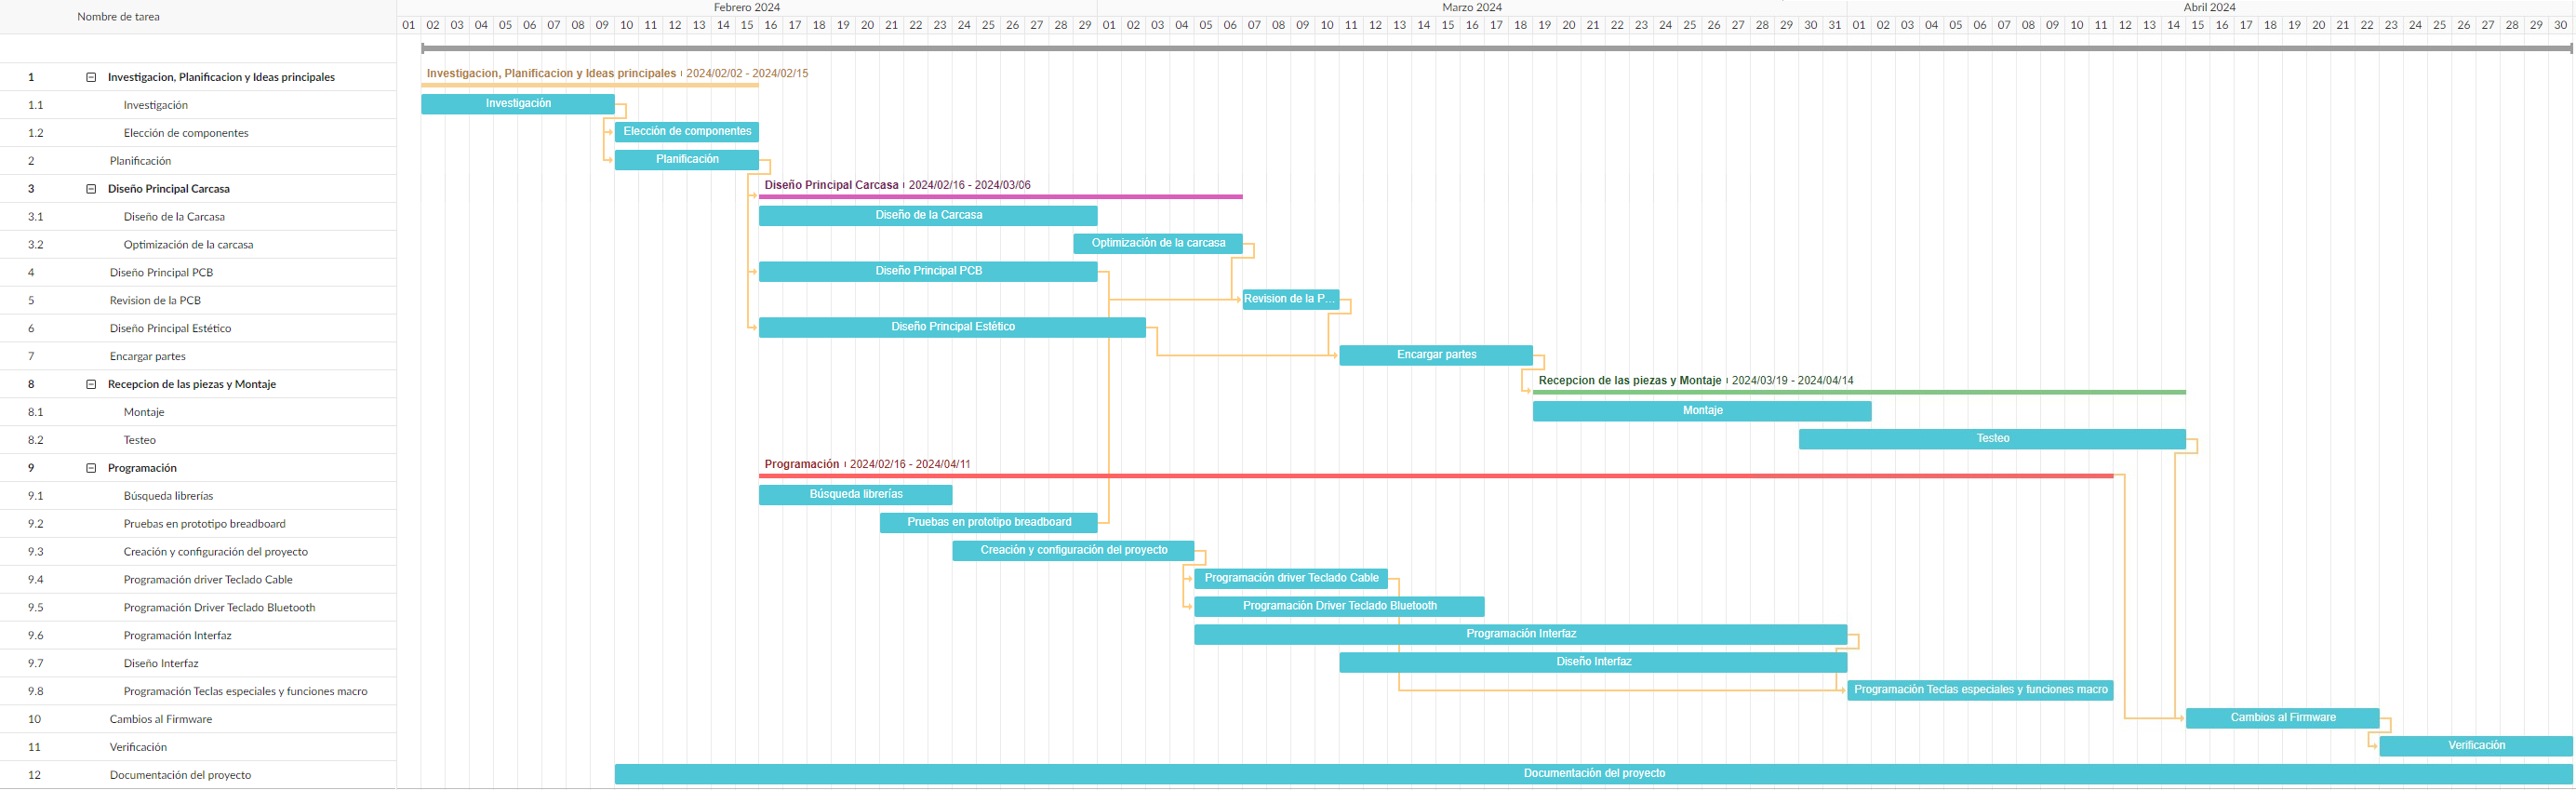
\includegraphics[width=\textheight]{imagenes/Capitulos/Cap02/DiagramaGantt.png}
\caption{Planificación del proyecto con diagrama Gantt.}
\label{fig:DiagramaGantt}
\end{sidewaysfigure}
